\begin{frame}[label=opening]{Darcy Problem}
    \frametitle{Opening}
    \framesubtitle{Darcy Problem}
    \begin{columns}[T]
        \begin{column}{.5\textwidth}
            \begin{figure}
                \centering
                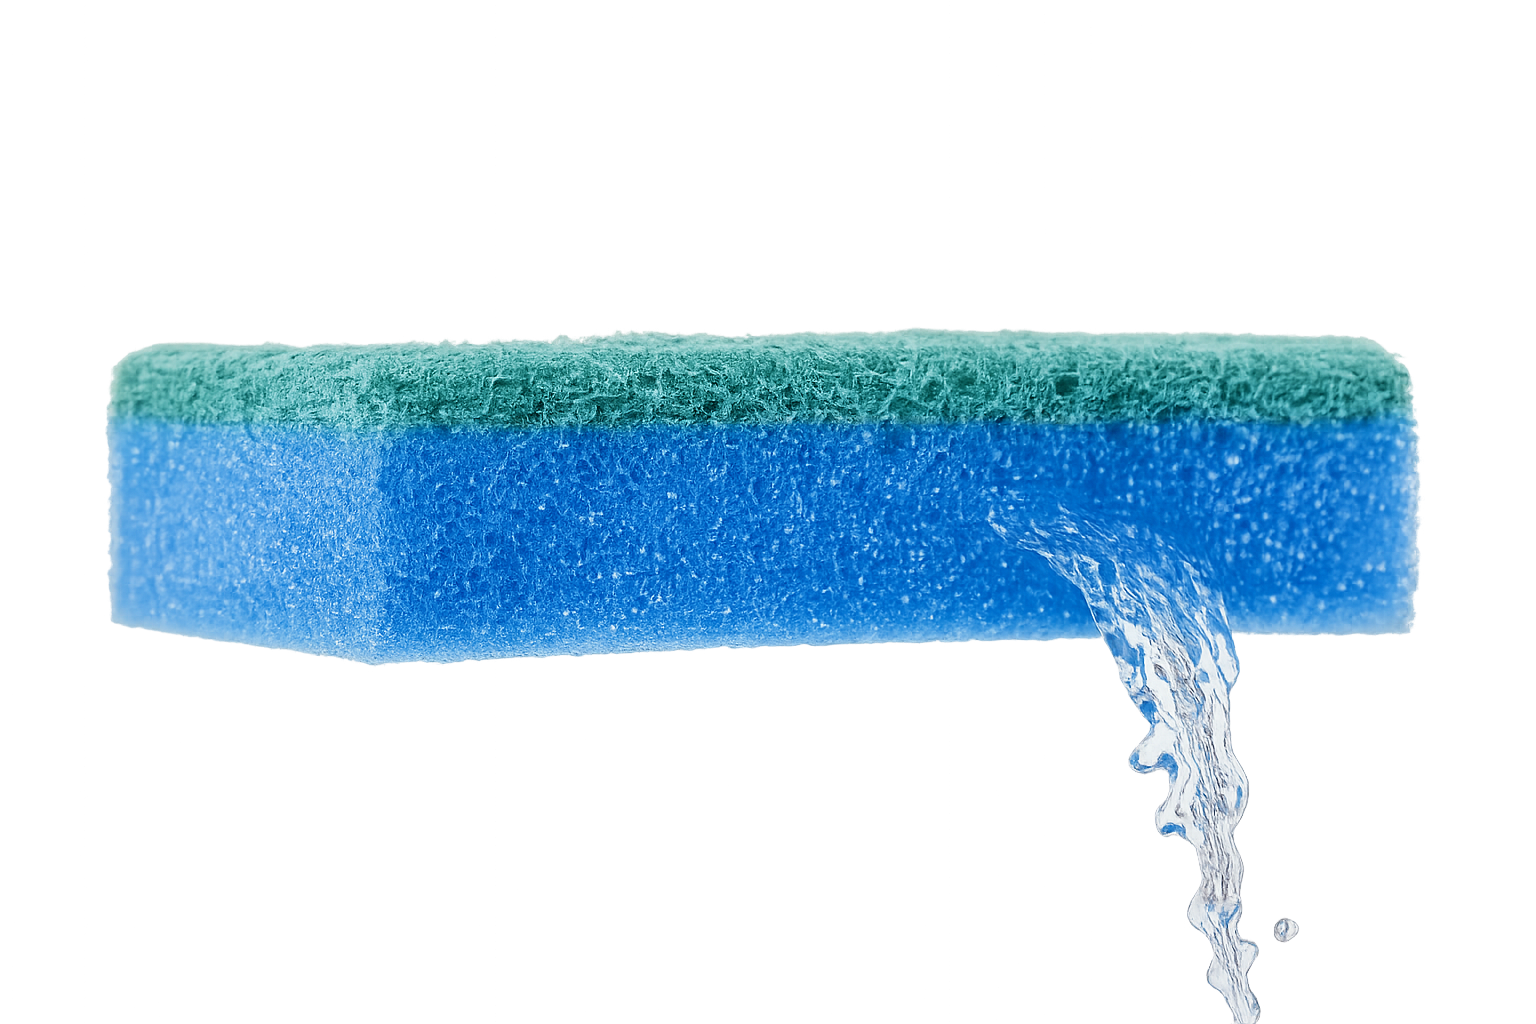
\includegraphics[width=\textwidth]{sponge.png}
            \end{figure}
        \end{column}
        \begin{column}{.5\textwidth}
            \begin{figure}
                \centering
                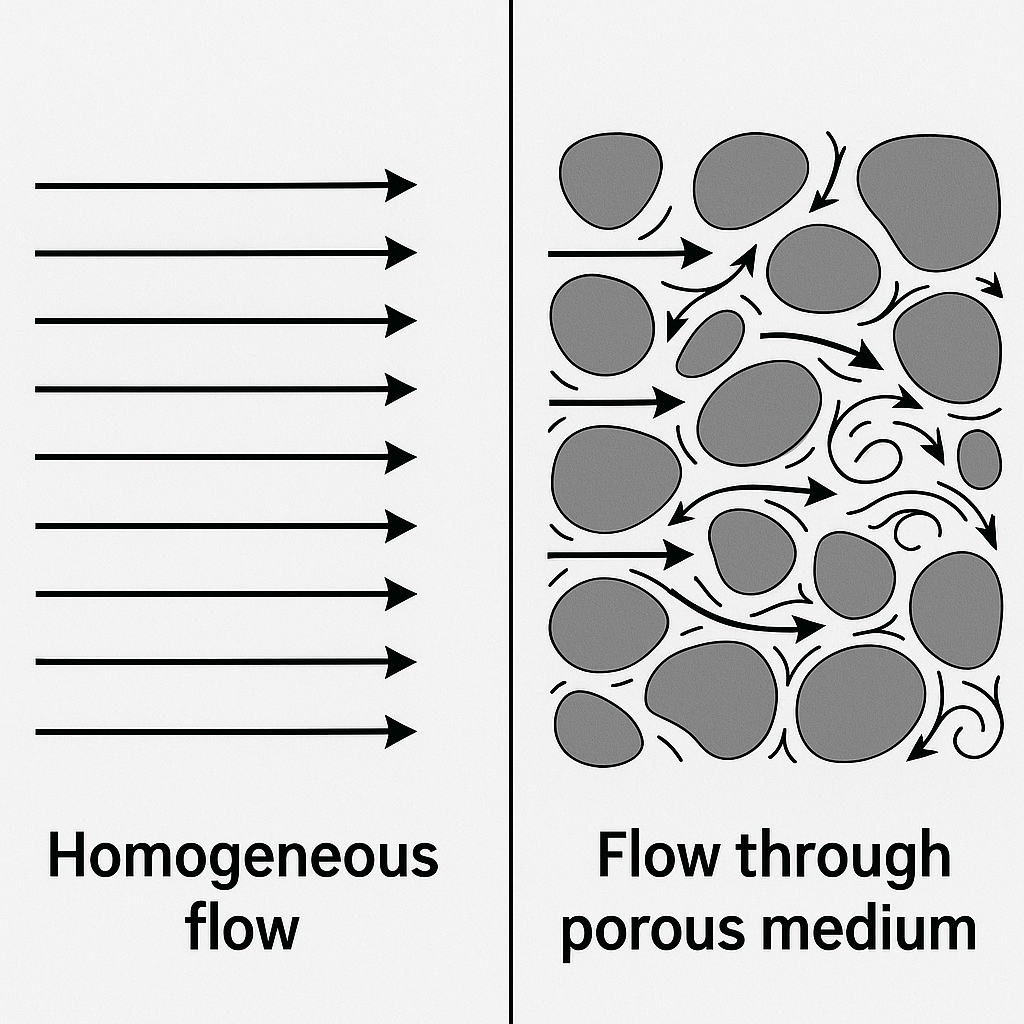
\includegraphics[width=0.8\textwidth]{homogeneous_vs_heterogeneous_flow.png}
            \end{figure}
        \end{column}
    \end{columns}
\end{frame}

% \begin{frame}[label=opening]{Conjugate Gradient Method}
%     \frametitle{Opening}
%     \framesubtitle{Conjugate Gradient Method}
% \end{frame}

% \begin{frame}[label=opening]{Condition Number}
%     \frametitle{Opening}
%     \framesubtitle{Condition Number}
% \end{frame}

% \begin{frame}[label=opening]{Preconditioners}
%     \frametitle{Opening}
%     \framesubtitle{Preconditioners}
% \end{frame}

% \begin{frame}[label=opening]{Research Gap}
%     \frametitle{Opening}
%     \framesubtitle{Research Gap}
% \end{frame}